% ================================================================
% Capitolul 5 – Aplicația
% Lucrare de licență: Kernel Trap – Sistem Inteligent de Prevenire
% a Intruziunilor cu Componente de Honeypot și Învățare Automată
% Autor: Banciu George-Horațiu
% Coordonator: Conf. Univ. Dr. Bufnea Darius Vasile
% ================================================================

\chapter{Aplicația}

Capitolul de față descrie implementarea propriu-zisă a sistemului KernelTrap.
Structura urmează etapele clasice de dezvoltare software: enunțarea
cerințelor funcționale și nefuncționale, analiza pe scurt a problemei,
proiectarea arhitecturii și a fluxurilor cheie prin diagrame, descrierea
condensată a implementării pe componente și, în final, modul în care a fost
verificat sistemul.


\section{Cerințe}


Funcționalitățile vizate au fost transpuse în cerințe specifice, prezentate
în tabelele \ref{tab:cap5-fr} și \ref{tab:cap5-nfr}. Acestea constituie
referința în raport cu care sistemul a fost evaluat în capitolul \ref{tab:cap6-perf}.

\begin{table}[h]
  \centering
  \caption{Cerințe funcționale}
  \label{tab:cap5-fr}
  \renewcommand{\arraystretch}{1.08}
  \begin{tabular}{|c|p{0.78\textwidth}|}
    \hline
    \textbf{ID} & \textbf{Descriere} \\
    \hline\hline
    FR1 & Agentul colectează în timp real evenimentele de syscall produse pe gazdă și le publică pe serverul central, filtrând automat sesiunile SSH active. \\
    \hline
    FR2 & Serverul central atribuie un scor fiecărui eveniment printr-un model Isolation Forest pre-antrenat și calibrat per-(gazdă, utilizator). \\
    \hline
    FR3 & Sistemul declanșează automat pivotarea unei sesiuni SSH suspecte către containerul honeypot, fără ca atacatorul să sesizeze tranziția. \\
    \hline
    FR4 & Operatorul poate inspecta în timp real activitatea agenților și a utilizatorilor printr-un panou de control web. \\
    \hline
    FR5 & Operatorul poate declanșa manual pivotarea unui utilizator dintr-un buton din panou. \\
    \hline
    FR6 & Containerul honeypot înregistrează integral sesiunea atacatorului și raportează evenimentele înapoi în panou. \\
    \hline
  \end{tabular}
\end{table}

\begin{table}[h]
  \centering
  \caption{Cerințe nefuncționale}
  \label{tab:cap5-nfr}
  \renewcommand{\arraystretch}{1.08}
  \begin{tabular}{|c|p{0.78\textwidth}|}
    \hline
    \textbf{ID} & \textbf{Descriere} \\
    \hline\hline
    NF1 & Overhead la nivelul gazdei monitorizate sub 2,5\% din CPU, măsurat în condiții de încărcare medie. \\
    \hline
    NF2 & Latența între producerea evenimentului declanșator și emiterea comenzii de pivotare sub o secundă. \\
    \hline
    NF3 & Sistemul tolerează căderi temporare ale serverului central; agenții continuă să publice și serverul reia procesarea fără pierdere de evenimente. \\
    \hline
    NF4 & Adăugarea unei gazde noi nu necesită nicio modificare a serverului central (zero-configuration discovery). \\
    \hline
  \end{tabular}
\end{table}


\section{Analiză}


Cerințele enunțate mai sus împart sistemul în patru responsabilități clar
separate: \emph{colectarea} datelor (FR1), \emph{analiza} și \emph{decizia}
de pivotare (FR2, FR3), \emph{izolarea} atacatorului (FR3, FR6) și
\emph{observabilitatea} pentru operator (FR4, FR5). Combinate cu cerințele
de performanță și de decuplare (NF1--NF4), aceste responsabilități exclud
varianta unei aplicații monolitice și favorizează o arhitectură distribuită
orientată pe evenimente, în care componentele comunică prin mesaje păstrate
într-o magistrală comună, nu prin apeluri sincrone directe. Motivele
detaliate ale acestei alegeri, împreună cu justificarea fiecărei tehnologii
folosite, au fost expuse în capitolul anterior (Abordarea propusă); secțiunile
care urmează tratează modul concret în care arhitectura este pusă în practică.


\section{Proiectare}


Această secțiune prezintă structural sistemul prin trei figuri:
arhitectura de componente (figura \ref{fig:cap5-arch}), fluxul de detecție
și pivotare (figura \ref{fig:cap5-seq-pivot}) și distribuția scorurilor de
normalitate produse de model (figura \ref{fig:cap5-scores}).

\textbf{Arhitectura de componente.} Sistemul este organizat în trei zone
funcționale, conectate exclusiv prin magistrala Redis Streams: gazda
monitorizată (unde rulează agentul și sursa de telemetrie Tracee), serverul
central (cu modulul de atribuire a scorului, fereastra glisantă și interfața
de control) și containerul honeypot (cu propriul mecanism de monitorizare).
Săgețile din figura~\ref{fig:cap5-arch} indică direcția și mijlocul de
comunicare folosit între componente: scrierea și citirea evenimentelor pe
stream-urile Redis (operațiile \texttt{XADD} și \texttt{XREAD}), apelurile
HTTP și conexiunea WebSocket dinspre serverul FastAPI către panoul de control,
iar la nivel local pe gazdă semnalul \texttt{SIGUSR1} (folosit pentru a
declanșa trap-ul de pivotare din shell-ul atacatorului) și regulile
\texttt{iptables} (pentru blocarea conexiunilor de la IP-ul atacatorului).

\begin{figure}[!htb]
  \centering
  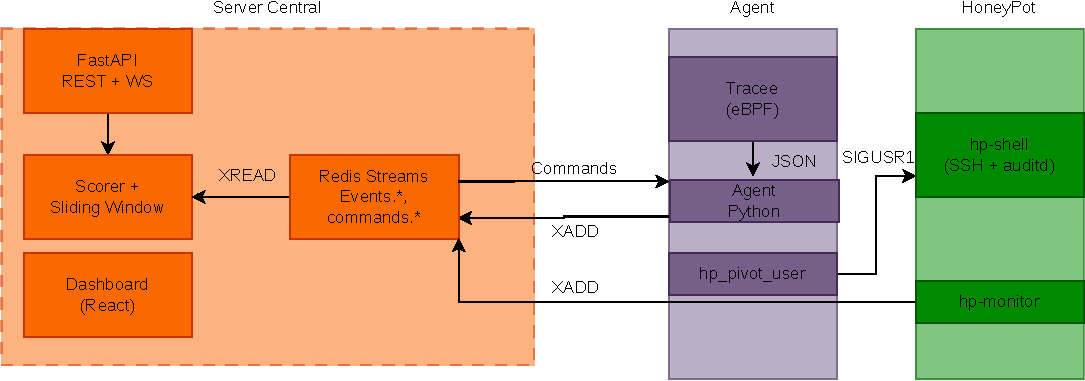
\includegraphics[width=\textwidth]{figuri/cap5-arch.pdf}
  \caption[Arhitectura de componente]{Arhitectura de componente. Cele trei zone comunică
           exclusiv prin Redis Streams; serverul central agregă fluxurile,
           atribuie scoruri și emite comenzi de pivotare.}
  \label{fig:cap5-arch}
\end{figure}

\textbf{Fluxul de pivotare.} Diagrama de secvență din figura~\ref{fig:cap5-seq-pivot}
urmărește calea completă a unui eveniment, de la momentul în care Tracee
îl captează pe gazdă, până la momentul în care shell-ul atacatorului este
înlocuit cu o sesiune SSH către container. Sunt evidențiate patru tranziții
cheie: publicarea evenimentelor în loturi pe magistrală, atribuirea scorurilor și
agregarea în fereastra glisantă, emiterea comenzii de pivotare către gazda
afectată și, în final, execuția pe gazdă a scriptului de pivotare, care
realizează în paralel trei sub-acțiuni: blocarea conexiunilor cu
\texttt{iptables}, provizionarea contului oglindit în container și trimiterea
semnalului \texttt{SIGUSR1} care comută efectiv sesiunea.

\begin{figure}[h]
  \centering
  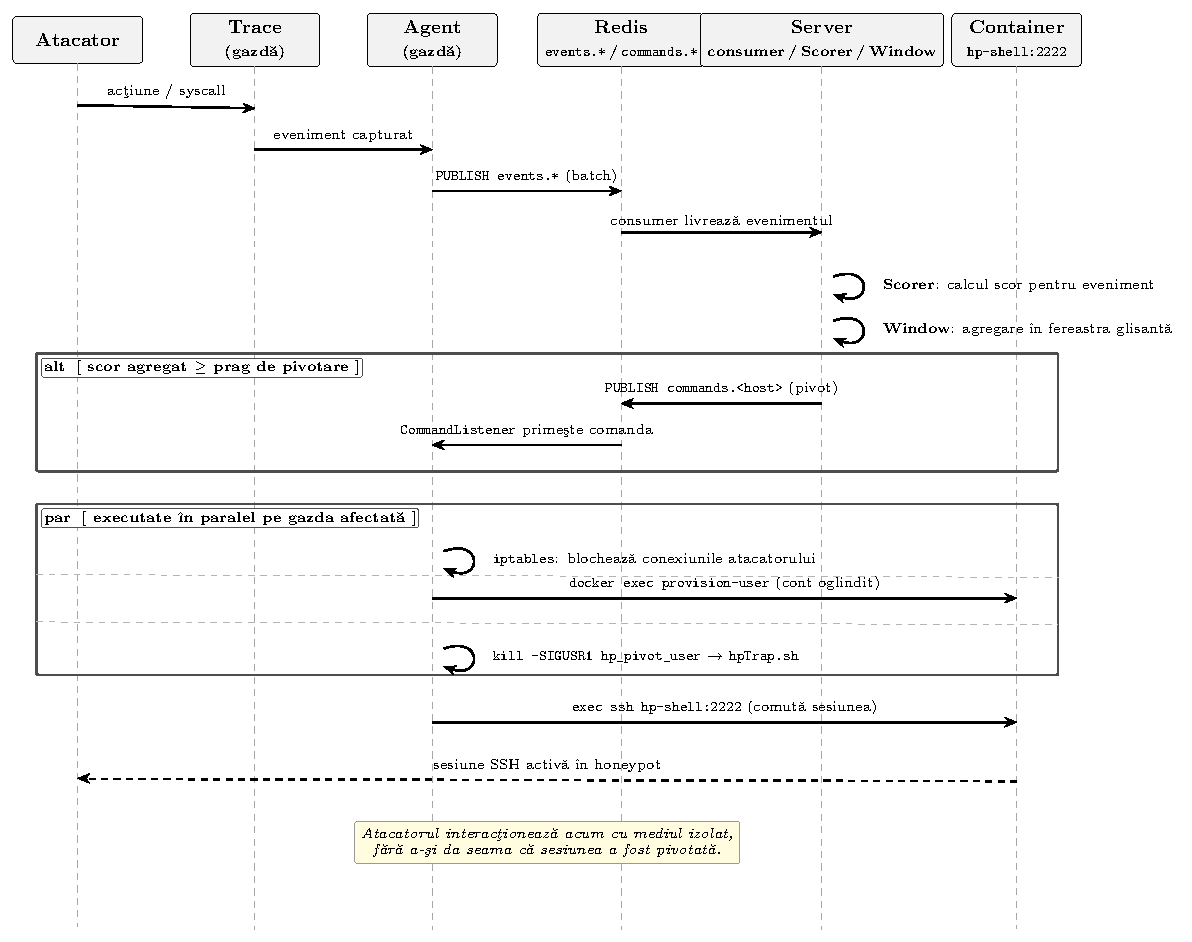
\includegraphics[width=\textwidth]{figuri/cap5-seq-pivot.pdf}
  \caption{Diagrama de secvență a procesului de detecție și pivotare}
  \label{fig:cap5-seq-pivot}
\end{figure}

\textbf{Distribuția scorurilor de normalitate.} Pentru fiecare eveniment,
modelul Isolation Forest emite un scor continuu: valorile pozitive corespund
comportamentului considerat normal, iar cele negative anomaliilor (cu cât
scorul este mai aproape de $-1$, cu atât evenimentul este mai izolat de
restul datelor benigne văzute la antrenare). Figura~\ref{fig:cap5-scores}
ilustrează distribuția acestor scoruri pe partiția de calibrare, cu cele
două praguri marcate vertical: percentila 2,0\% ($s = -0{,}022$, severitate~1)
și percentila 0,2\% ($s = -0{,}102$, severitate~2). Cele trei zone rezultate
(benign, minor și major) corespund direct nivelurilor de severitate pe baza
cărora fereastra glisantă cumulează indicii și decide când să declanșeze
pivotarea.

\begin{figure}[h]
  \centering
  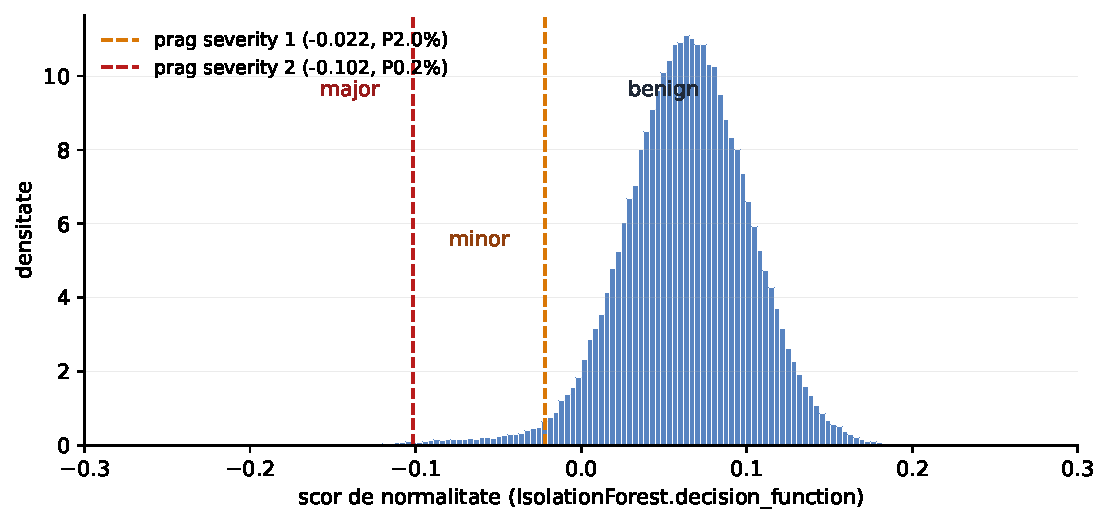
\includegraphics[width=0.85\textwidth]{figuri/cap5-scores.pdf}
  \caption[Distribuția scorurilor Isolation Forest]{Distribuția ilustrativă a scorurilor de normalitate produse de
           IsolationForest, cu pragurile de severitate 1 și 2 marcate.}
  \label{fig:cap5-scores}
\end{figure}


\section{Implementare}


\subsection{Tehnologii și organizarea proiectului}

Sistemul este împărțit în patru componente software, fiecare adaptată 
rolului pe care îl ocupă (tabelul~\ref{tab:cap5-stack}).
Alegerile principale sunt motivate de cerințele nefuncționale: framework-ul
web FastAPI împreună cu serverul \texttt{uvicorn} oferă concomitent un API
REST și un canal WebSocket asincron pe aceeași conexiune; biblioteca
scikit-learn pune la dispoziție o implementare matură și bine optimizată
a algoritmului Isolation Forest; Tracee permite instrumentarea kernelului
prin eBPF fără să fie nevoie de recompilarea pe fiecare versiune de kernel
țintă, iar Redis Streams oferă o magistrală de mesaje persistentă, suficient de
robustă pentru cazurile de utilizare ale sistemului, fără a impune
complexitatea operațională a unui sistem dedicat de mesagerie de tip Kafka
sau RabbitMQ.

\begin{table}[h]
  \centering
  \caption{Stiva tehnologică pe componente}
  \label{tab:cap5-stack}
  \renewcommand{\arraystretch}{1.08}
  \begin{tabular}{|l|l|}
    \hline
    \textbf{Componentă} & \textbf{Tehnologii} \\
    \hline\hline
    Agent de colectare        & Python 3, Tracee (\texttt{aquasec/tracee:latest}), \texttt{redis-py} \\
    \hline
    Server central            & Python 3, FastAPI, uvicorn, scikit-learn, NumPy \\
    \hline
    Container honeypot        & Docker (Ubuntu 22.04), OpenSSH, \texttt{auditd}, \texttt{util-linux} \\
    \hline
    Panou de control          & React 19, Vite 5, WebSocket \\
    \hline
    Mesagerie                 & Redis 7 (Streams) \\
    \hline
    Container runtime         & Docker (\texttt{docker.io}) \\
    \hline
  \end{tabular}
\end{table}

Repository-ul este organizat pe componente, cu două scripturi de instalare 
care ascund detaliile de inițializare:

\begin{lstlisting}[caption={Structura repository-ului (esențială)}, label={lst:cap5-tree}]
KernelTrap/
  central_server/         # Serverul central FastAPI + scorer + window
    main.py, scorer.py, window_v3.py, requirements.txt
  masina_invata/
    isolation_forest/     # Antrenare Isolation Forest pe BETH
    logger/               # Agentul (syscall_logger.py)
  Honeypot/               # Imagine Docker honeypot + script pivotare
    Dockerfile, hp_pivot_user.sh, hpTrap.sh
    provision-user.sh, record-session.sh, start-sshd.sh
    hp-monitor.py, install.sh
  dashboard/              # Aplicatie React + Vite (panoul de control)
  start_server.sh         # Bootstrap server central + Redis + dashboard
  start_agent.sh          # Bootstrap agent pe gazda monitorizata
\end{lstlisting}

\subsection{Componente}

\textbf{Agentul} este componenta care rulează pe fiecare gazdă protejată.
Primește în timp real evenimentele de syscall capturate de Tracee, le aduce
într-un format uniform (inclusiv conversia numelor de syscall în identificatori
numerici stabili, pentru a putea fi tratate consistent de modelul de
învățare automată) și le trimite serverului central în loturi, prin magistrala
Redis. Pentru a reduce zgomotul, păstrează doar evenimentele provenite de la
utilizatori conectați activ prin SSH și elimină propriile sale apeluri.
Un al doilea fir de execuție așteaptă în paralel comenzi de la server: când
primește o decizie de pivotare, lansează scriptul corespunzător pentru a
redirecționa sesiunea atacatorului în honeypot. La nivel de implementare,
toată această logică este concentrată în
\texttt{masina\_invata/logger/syscall\_logger.py}, cu clasele
\texttt{TraceeParser} (parsing) și \texttt{CommandListener} (firul de
ascultare a comenzilor), folosind biblioteca \texttt{redis-py} pentru
comunicația cu magistrala.

\textbf{Serverul central} este creierul sistemului: agregă fluxurile de la
toți agenții, atribuie un scor fiecărui eveniment și decide când o sesiune
trebuie pivotată. Activitatea este împărțită în patru sarcini care rulează
în paralel: prima consumă evenimentele primite de la agenți, a doua le atribuie un scor
și actualizează fereastra glisantă, a treia publică deciziile de pivotare înapoi
către gazde, iar ultima menține panoul de control la zi prin WebSocket.
Modulele care implementează aceste responsabilități sunt
\texttt{central\_server/main.py} (orchestrarea celor patru sarcini asincrone
peste un server FastAPI), \texttt{central\_server/scorer.py} (clasa
\texttt{Scorer}, care încapsulează modelul Isolation Forest împreună cu
pipeline-ul celor 22 de caracteristici și lexicoanele de procese
cunoscute) și \texttt{central\_server/window\_v3.py} (clasa
\texttt{SlidingWindowTracker}, care aplică pragul dublu cantitate + rată).
Modelul antrenat salvat în trei fișiere
(\texttt{iforest.joblib}, \texttt{scaler.joblib}, \texttt{meta.json}) este
încărcat în memorie o singură dată la pornire, dintr-un director versionat
împreună cu sursa.

\textbf{Mecanismul de pivotare} traduce o decizie a serverului în acțiunea
concretă de redirecționare a sesiunii atacatorului. Este realizat din două
scripturi shell complementare. Primul, \texttt{hp\_pivot\_user.sh} (instalat
în \texttt{/usr/local/sbin} cu o regulă \texttt{sudoers} care permite agentului
să-l ruleze fără parolă), execută în ordine trei acțiuni: blochează
conexiunile noi de la IP-ul atacatorului printr-o regulă \texttt{iptables},
provizionează contul corespunzător în containerul honeypot prin
\texttt{docker exec provision-user.sh}, apoi trimite semnalul
\texttt{SIGUSR1} către shell-urile active ale utilizatorului. Al doilea,
\texttt{hpTrap.sh}, este livrat ca fragment din \texttt{/etc/profile.d/}
și se încarcă automat în fiecare shell interactiv la login; instalează un
\textit{trap} care, la primirea semnalului \texttt{SIGUSR1}, înlocuiește
procesul curent al shell-ului cu o sesiune SSH către container, fără ca
utilizatorul să observe tranziția:

\begin{lstlisting}[caption={Trap-ul instalat în fiecare shell interactiv (\texttt{hpTrap.sh})}, label={lst:cap5-trap}]
hptrap_pivot() {
  logger -t hptrap "Pivoting user $USER from host to honeypot"
  exec ssh -i /etc/hptrap/hp_key -o StrictHostKeyChecking=no \
    "${USER}@127.0.0.1" -p 2222
}
trap hptrap_pivot USR1
\end{lstlisting}

\textbf{Containerul honeypot} oferă un mediu Linux aparent obișnuit, în
care atacatorul ajunge după pivotare. Imaginea de bază este \texttt{ubuntu:22.04}
cu server SSH, auditare la nivel de kernel (\texttt{auditd}) și utilitarele
uzuale de linie de comandă. La momentul pivotării, un script de
provizionare creează automat în container un cont oglindit (cu același nume
ca pe gazda reală) și populează directorul home al acestuia cu fișiere-momeală
plauzibile: chei AWS, o cheie SSH privată, un fișier de mediu cu credențiale
fictive de bază de date, note interne și un token CI/CD. Toate aceste fișiere
sunt urmărite de \texttt{auditd}: orice citire sau scriere asupra lor generează
imediat un eveniment. Pe lângă canary-uri, sesiunea integrală a atacatorului
este înregistrată ca tranzit TTY, iar un script de monitorizare
(\texttt{hp-monitor.py}) citește continuu log-ul \texttt{auditd} și publică
evenimentele înapoi pe magistrala Redis, în același format folosit de agenții
de pe gazdele reale, astfel încât panoul de control le poate afișa unitar,
indiferent de sursă.

\textbf{Panoul de control} este o aplicație web scrisă în React, păstrată
deliberat minimală (singurele dependențe runtime sunt \texttt{react} și
\texttt{react-dom}). Comunică cu serverul central pe două căi: un API REST
pentru date relativ statice (lista agenților, istoric pivotări) și o conexiune
WebSocket pentru fluxul live de evenimente. Reconectarea automată cu
\textit{backoff} exponențial (creșterea progresivă a intervalului dintre
încercări) este gestionată centralizat printr-un singur \textit{hook}
custom, astfel încât celelalte componente pot presupune că au date la zi.
Vizual, panoul este împărțit în patru zone: lista agenților conectați
(\texttt{AgentsPanel}), fluxul de log-uri în timp real (\texttt{LiveLogs}),
tabelul utilizatorilor monitorizați cu progresul în fereastra glisantă
(\texttt{UsersTable}) și istoricul pivotărilor (\texttt{PivotHistory}).
Aplicația este compilată ca site static și servită direct de serverul
FastAPI, eliminând nevoia unui server web separat.

\textbf{Antrenarea modelului} se realizează offline, înainte de punerea
în funcțiune a sistemului, pe partiția benignă a setului de date BETH.
Pentru a putea folosi întregul volum de date disponibil (zeci de gigabytes),
fără a-l încărca complet în memorie, se folosește o tehnică de eșantionare
numită \textit{reservoir sampling}: pe măsură ce datele sunt citite în
\textit{streaming}, un eșantion uniform de dimensiune fixă este menținut și
actualizat probabilistic. Concret, modelul folosit în producție este antrenat
pe 10 milioane de instanțe astfel eșantionate, cu o pădure de 2000 de arbori
de izolare. Pragurile de severitate 1 și 2 nu sunt fixate arbitrar, ci sunt
calibrate ulterior pe o partiție de validare, alegând percentilele 2,0\% și
0,2\% ale scorurilor de normalitate, astfel încât proporția de evenimente
marcate ca anomalii pe date benigne să fie controlată explicit. Aceste praguri,
împreună cu tabelele de codificare prin frecvență ale câmpurilor categoriale,
sunt salvate în \texttt{meta.json} și citite la pornirea serverului central.
Scriptul de antrenare se află în
\texttt{masina\_invata/isolation\_forest/beth\_iforest.py}.


\section{Testare}


Sistemul a fost validat prin cinci tipuri complementare de testare,
descrise pe scurt mai jos. Rezultatele cantitative în special cele
referitoare la detecția scenariilor reale de atac sunt prezentate detaliat
în capitolul~\ref{tab:cap6-perf}.

\textbf{Testarea modelului de învățare automată.} Scriptul de antrenare
expune o subcomandă dedicată de evaluare care încarcă modelul deja antrenat
împreună cu partiția de test a setului BETH, calculează scorurile, aplică
pragurile de severitate calibrate și raportează două metrici de referință
asupra atacurilor etichetate: aria de sub curba ROC (\texttt{roc\_auc\_evil})
și precizia medie (\texttt{avg\_precision\_evil}). Acest test este reluat
la fiecare reantrenare, ca o regresie de calitate care semnalează imediat
dacă o nouă versiune a modelului pierde din capacitatea de detecție.

\textbf{Teste unitare pe componentele critice ale serverului.} Cele două
clase cu logică algoritmică sensibilă \texttt{Scorer} și
\texttt{SlidingWindowTracker} sunt acoperite de teste unitare \texttt{pytest}
(\texttt{tests/test\_scorer.py} și \texttt{tests/test\_window.py}). Pentru
\texttt{Scorer} sunt verificate încărcarea corectă a modelului,
schema evenimentelor procesate și comportamentul pe input
degenerat (lot gol). Pentru \texttt{SlidingWindowTracker} sunt verificate
condițiile fundamentale ale pragului dublu: nici un pivot sub prag, pivotare
exact când cantitatea și rata sunt simultan satisfăcute, blocarea pivotării
când rata este sub limită (chiar dacă numărul de evenimente severe e mare),
ignorarea UID-urilor omise și suprimarea pivotărilor repetate imediat
după un pivot deja declanșat.

\textbf{Testare de integrare end-to-end.} Cea mai relevantă verificare
practică se face prin rulări controlate ale întregului sistem: pornirea
simultană a serverului central (\texttt{start\_server.sh}) și a agentului
pe o gazdă de test (\texttt{start\_agent.sh}), generarea manuală de
activitate (autentificare SSH, comenzi controlate de recon) și observarea
în panoul de control că evenimentele apar, primesc scor, fereastra glisantă
cumulează severitățile și, la pragul atins, pivotarea este efectiv
declanșată. O singură astfel de rulare exersează magistrala Redis Streams
în ambele direcții, scoring-ul, fereastra glisantă și mecanismul de pivotare.

\textbf{Testarea mecanismului de pivotare și a honeypot-ului.} Pivotarea
este verificată suplimentar prin invocare directă din linia de comandă:
\texttt{sudo hp\_pivot\_user <username>} într-o sesiune SSH activă.
Se confirmă apariția regulii \texttt{iptables} (vizibilă cu
\texttt{iptables -L INPUT -n}), tranziția shell-ului către container
(PID-ul shell-ului inițial este înlocuit) și prezența fișierelor-momeală
în directorul home oglindit. Înregistrarea integrală a sesiunii este
verificată prin inspecția fișierelor din \texttt{/var/log/sessions/} ale
containerului, iar regulile de auditare sunt validate prin acces deliberat
la fișierele-capcană și observarea evenimentelor corespunzătoare în panou.

\textbf{Testarea panoului de control.} Interfața web este verificată
manual în browser: indicatorul de status al serverului (verde/roșu),
fluxul de evenimente prin WebSocket, tabelul utilizatorilor cu progresul
ferestrei glisante și declanșarea unui pivot prin butonul dedicat.
Reconectarea automată cu \textit{backoff} exponențial este verificată prin
oprirea voluntară a serverului în timpul rulării panoului clientul se
reconectează la repornirea serverului, fără intervenție manuală.

Această combinație a fost preferată unei suite extinse de teste unitare pe
toate componentele: întrucât sistemul este distribuit și comunică exclusiv
prin Redis Streams, comportamentul realist apare doar la integrare. Testele
unitare au fost menținute strict acolo unde logica este suficient de izolată
și de critică pentru a justifica izolarea în Scorer și în fereastra glisantă 
iar restul componentelor sunt acoperite de testele de integrare end-to-end.
